\section{Introduction}

Speculative bubbles are perceived to periodically take over markets \cite{garber2001famous}.
Going back at least to the \emph{South Sea} bubble in the early 18$^{\text{th}}$ century, well-informed parties  have invested knowingly in bubbles, and found it profitable \cite{temin2004riding}.
Today, the public notoriety of Bitcoin, together with its massive price increases and their associated publicity lead to an explosion of attempts to create ``the next Bitcoin''.
Collectively, these currencies are often referred to as ``cryptocurrencies'' or simply ``coins'', and a vibrant set of exchanges have emerged where these are traded, either for each other or money.
The majority of these coins have no possible future valuable in the long term, and their markets would appear to be driven largely by speculation.
Many of them appear to be nothing but attempts at turning a quick profit from inflating the implied valuation of a coin shortly after creating it.
This is driven by the extremely low cost and effort required to create a new coin, with most being minimal changes to parameters and branding of a pre-existing codebase.

Those who make and trade these coins communicate largely online, and much of their activity is concentrated on public forums. 
As such, price and volume data from these exchanges is freely available and widely aggregated\footnote{ these are however largely unregulated, often anonymous, and there is no way to account how much of reported volumes are manipulation attempts. The existence of attempts at arbitrage between them places some bounds on how blatantly the data can be manipulated for prices, but volumes are impossible to assess. },
%JULIAN: Whole footnote is one extra-long sentence!
and the source code to all of them being public is the norm%\footnote{cargo cult CS being derigour in the comunity}.
. This makes cryptocoins
%JULIAN: cryptocoins is a new work--maybe avoid mixing the terms
an ideal lens through which to study the social life of a ``market mania'' \cite{cosma2008}.
Such a study is valuable both as a means of understanding the dynamics of bubbles themselves, but also from a computational social science perspective, to understand the ecosystem and lifecycles of these online communities.
%Such a study can serve in the computational social sciences a role analogous to that of lesion studies do in neuropsychology.
%JULIAN: Not obvious to me what the above analogy is without further explanation.


%\begin{figure}[h!]
%\end{figure}

We present a study of a large number of cryptocurrency ecosystems, 
using a novel dataset that combines measures derived from social networks of users in cryptocurrency forums, market data aggregated over dozens of exchanges, and properties of the software implementing the cryptocurrencies themselves.
From forums we identify the introducers of each coin and build measures of their position in the network based on
%which users have engaged with them
their patterns of engagement in forum threads
%threads in the forum
\emph{before} the coin is announced.
In this way we identify 376 coins that are announced by users of the forum and which can be mapped to price and volume data from exchanges.
Next, from price and transaction volume data we build measures of the subsequent activity that results from trading in the coin. 
We also assess if coins possibly embody technological innovation based on having more than trivial modifications to previously existing coins' source code.


%\begin{figure}
%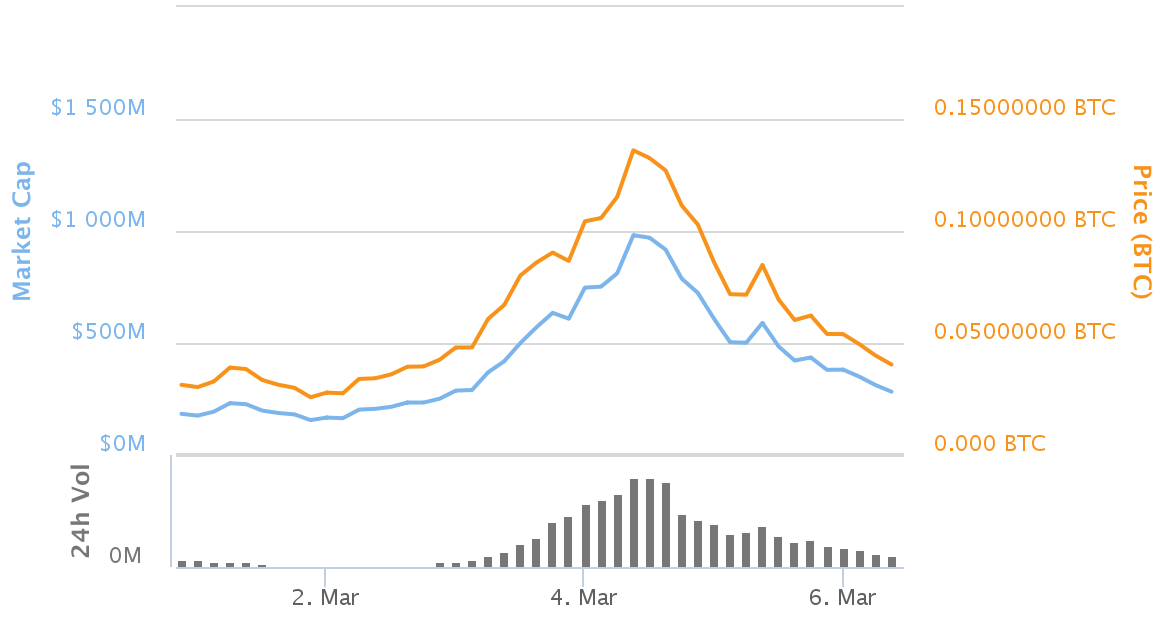
\includegraphics[width=\columnwidth]{AuroraCoin}
%\end{figure}

While the mechanisms that drive bubbles have been studied both theoretically 
\cite{abolafia1988enacting, earl2007decision, bakker2010social, harras2011grow}
and experimentally
\cite{moinas2013bubble},
% in the lab, 
an exhaustive dataset and study of the social networks of those promoting the asset has not been previously previously possible.
While the magnitude of the assets traded is certainly small relative to most financial and commodity markets, it is nevertheless much larger than
%JULIAN: Found this sentence a bit funny, not that I could improve upon it
even the most lavishly funded experimenter could hope for.
For example, the largest bubble in our dataset, AuroraCoin, reaches a valuation of one billion USD in March 2014,
with reported daily trading volumes of 6.8M USD, and sheds 90\% of its value in a week, and 99\% of its value in well under a year.
For context, this is equivalent to one quarter of Iceland's entire foreign exchange reserves in 2014,\footnote{4.1 Billon USD, The World Bank, Global Economic Monitor, accessed October 2015} the population of which AuroraCoin promoters claimed they would distribute half of the coins to.

\begin{figure}
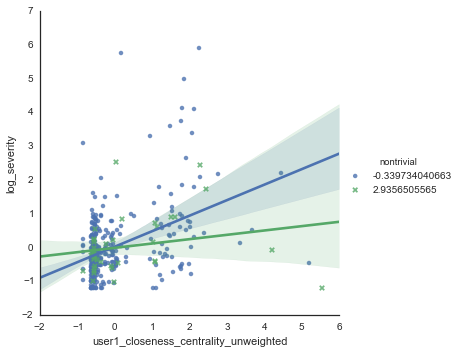
\includegraphics[width=\columnwidth]{severity_centrality}
\end{figure}

Using price and volume data we construct measures of both the magnitude and the severity of bubbles.
These are defined formally in our variable section,
%JULIAN: Give a section ref?
but their intuition is that we say the magnitude of a coin is large when a high volume in dollars of trades happens,
%JULIAN: Does it make a difference what it's measured in?
while we say a coin has a severe bubble if investing a fixed amount leads to loosing a large proportion. 
By considering the community structure that exists in the forum before a coin is introduced we are able to predict a substantial fraction of the variation in both the severity and magnitude of the resulting bubble.
This is a challenging task, and models that rely on either simple activity or network metrics metrics show almost no predictive out-of-sample power, unable to explain even 1\% of the variation in either task,
our best models perform an order of magnitude better in both tasks.
%JULIAN: R^2 of 0.1 (if I interpret correctly) doesn't sound impressive until you've argued the fundamental difficulty of the problem, you might wait to mention such numbers.
%JULIAN: Would sound more impressive if you just said "it performs an order of magnitude better"
The main driver of our explanatory power is the centrality of a user in the directed network derived from the forum. 
This effect appears to be mediated by whether a coin involves a nontrivial technological change, the direction of the interaction reversing depending on whether it relates to magnitude or severity.
%JULIAN: Above sentence is tough to parse, but kind of an important one.
Both the severity and the magnitude of bubbles increases with the centrality of the user who introduces the coins in the forums.  
Interestingly this effect is concentrated in different ways depending on whether the coin software is more than a trivial modification: trivial coins have more severe bubbles the more central their introducers are, while volume is greater the more central the introducer of a nontrivial coin is.




%JULIAN: Needs something outlining the paper's main results here, ideally a figure explaining the role of the various parts of the system.
%JULIAN: I'd tone down the footnotes

\begin{figure}
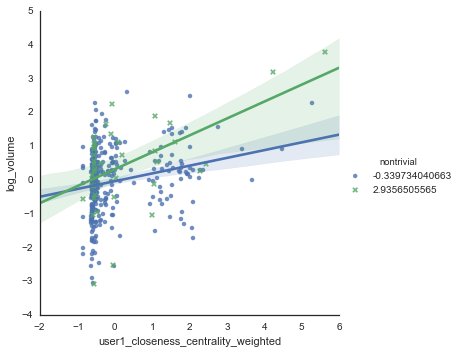
\includegraphics[width=\columnwidth]{volume_centrality}
\end{figure}

%Methodologically the free parameters in the way we do the weights on the weighted graph  is horrible, a million free parameters get introduced. follow up work for another paper: do some unsupervised feature learning over the dam forums threads to build the network; use some internal validity metric . Find political way of saying this in future work.
